\chapter{Related Work}
\label{Chapter-Related-Work}

% Todo: Edit to your liking
\section{Existing Batch-Processing Platforms}

\begin{figure}[h!]
  \centering
  \begin{subfigure}[b]{0.2\textwidth}
    
\includegraphics[width=\textwidth]{Images/airflow.png}
    % \caption{Apache Airflow}
    \label{fig:airflow}
  \end{subfigure}
  \begin{subfigure}[b]{0.3\textwidth}
    
\includegraphics[width=\textwidth]{Images/Apache_Spark_logo.svg.png}
    % \caption{Apache Spark}
    \label{fig:spark}
  \end{subfigure}
  \hfill
  \caption{Batch Processing Platforms}
  \label{fig:authservices}
\end{figure}

Batch-processing platforms are commonly used for running large-scale data workflows in analytics, ETL (Extract, Transform, Load), 
and machine learning pipelines. Examples include Apache Airflow~\cite{airflow}, Apache Spark~\cite{spark}, and Luigi~\cite{luigi}.

While these systems excel in orchestrating complex, DAG-based workflows~\cite{airflow-dag}, they typically assume a single system-level user or are 
operated by DevOps teams. They are not inherently designed to support multiple authenticated users submitting independent jobs with 
isolated resources.

In contrast, the system developed in this thesis places emphasis on user-level isolation, sandboxed execution, and seamless 
submission of containerized jobs without requiring workflow DSLs~\cite{fowler-dsl} or deep infrastructure knowledge.

\section{Data Lake Platforms}

\begin{figure}[h!]
  \centering
  \begin{subfigure}[b]{0.1\textwidth}
    
\includegraphics[width=\textwidth]{Images/awsLakeFormation.png}
    % \caption{AwsLake Formation}
    \label{fig:awslakeformation}
  \end{subfigure}
  \hfill
  \begin{subfigure}[b]{0.1\textwidth}
    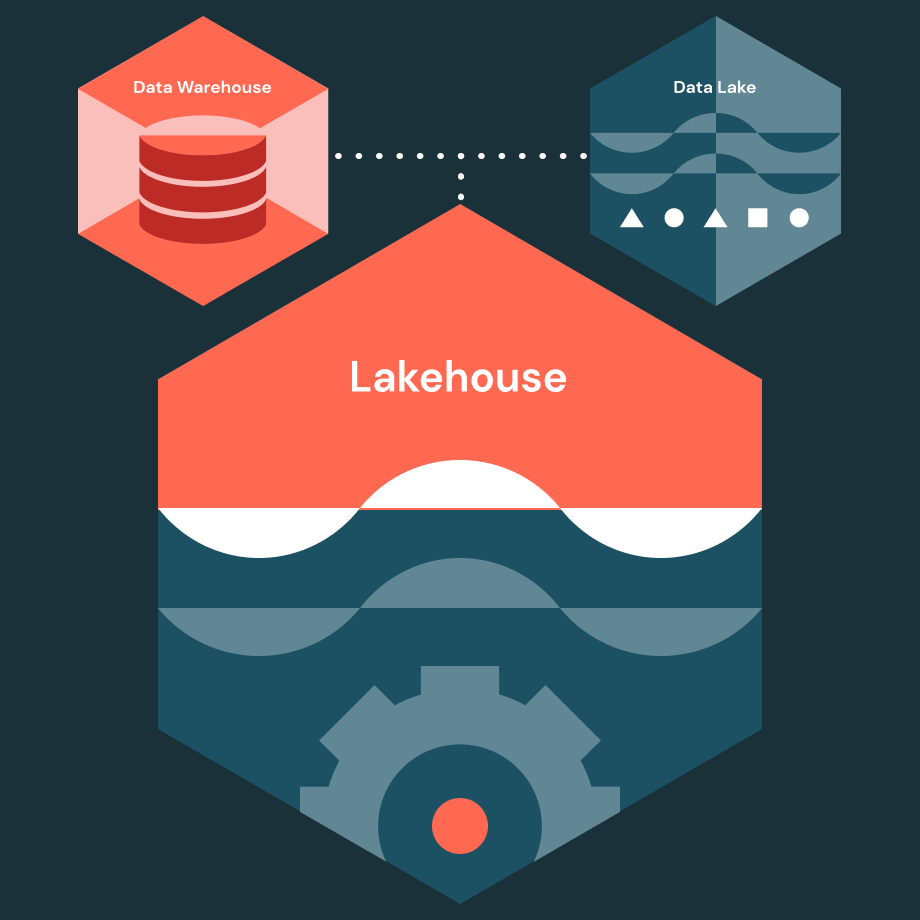
\includegraphics[width=\textwidth]{Images/LP-headerImage-lakehouse-architecture-2x.png}
    % \caption{DataBricks Lakehouse}
    \label{fig:databricks}
  \end{subfigure}
  \hfill
  \begin{subfigure}[b]{0.3\textwidth}
    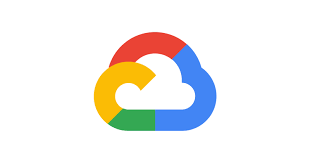
\includegraphics[width=\textwidth]{Images/google-cloud.png}
    % \caption{GoogleCloudBigLake}
    \label{fig:google}
  \end{subfigure}
  \caption{Data Lake Platforms}
  \label{fig:authservices}
\end{figure}

Data lake platforms such as AWS Lake Formation~\cite{aws-lake-formation}, Databricks Lakehouse~\cite{lakehouse}, 
and Google Cloud BigLake~\cite{biglake} provide unified storage and compute environments for large-scale data 
analytics. These platforms often integrate object storage, access control, and analytics tooling into a single 
managed service.

While they are powerful and mature, they are typically commercial, tightly integrated into specific cloud providers, and involve 
complex administrative overhead. Moreover, user-level job sandboxing and container-level compute customization are limited or 
highly abstracted.

The system described in this thesis aims to offer a lightweight, open alternative that provides user-level compute environments, 
shared storage, and access-controlled workflows within a Kubernetes-native ecosystem.

\section{Platform-as-a-Service Solutions}

\begin{figure}[h!]
  \centering
  \begin{subfigure}[b]{0.1\textwidth}
    
\includegraphics[width=\textwidth]{Images/heroku.png}
    % \caption{Heroku}
    \label{fig:heroku}
  \end{subfigure}
  \hfill
  \begin{subfigure}[b]{0.2\textwidth}
    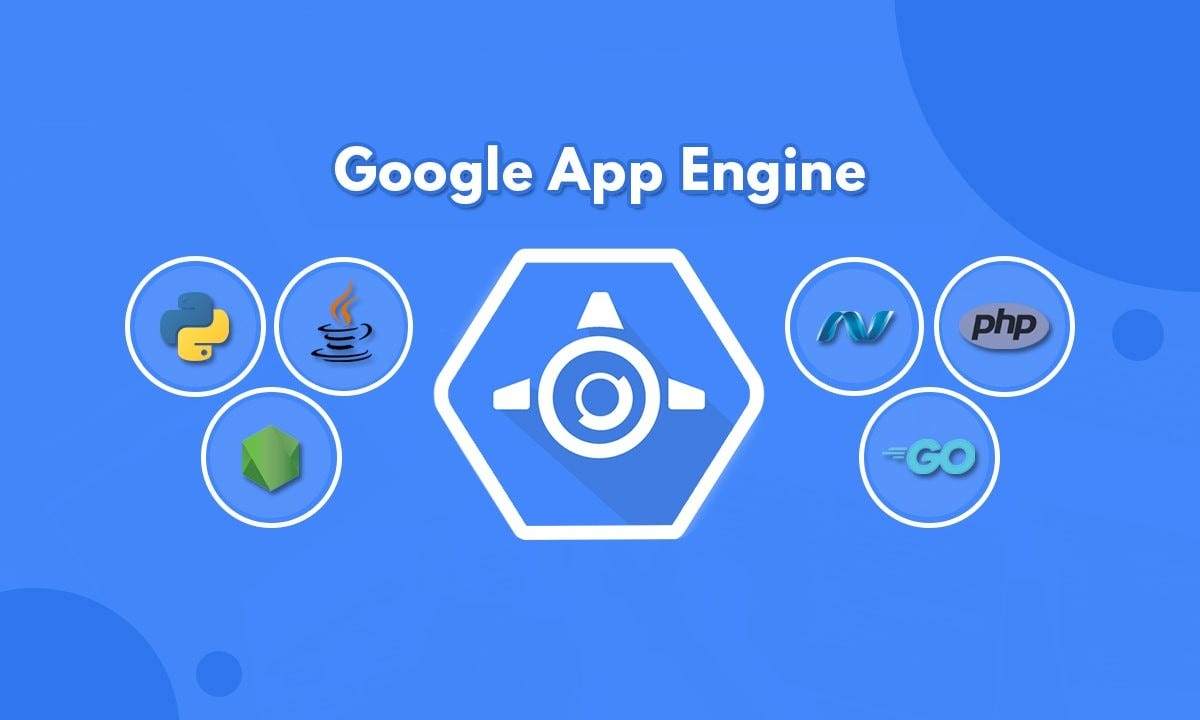
\includegraphics[width=\textwidth]{Images/google-app-engine.jpg}
    % \caption{GoogleAppEngine}
    \label{fig:gae}
  \end{subfigure}
  \hfill
  \begin{subfigure}[b]{0.3\textwidth}
    
\includegraphics[width=\textwidth]{Images/openshift.png}
    % \caption{OpenShift}
    \label{fig:openshift}
  \end{subfigure}
  \hfill
  \begin{subfigure}[b]{0.3\textwidth}
    
\includegraphics[width=\textwidth]{Images/jupyterhub.png}
    % \caption{JupyterHub}
    \label{fig:jupyterhub}
  \end{subfigure}

  \caption{PaaS}
  \label{fig:authservices}
\end{figure}

Platform-as-a-Service (PaaS)~\cite{nist-paas} offerings such as Heroku~\cite{heroku}, Google App Engine~\cite{appengine}, and OpenShift~\cite{openshift} enable developers to 
deploy and scale applications without managing infrastructure. Some educational platforms like JupyterHub~\cite{jupyterhub} 
provide multi-user notebooks for teaching and research purposes.

While JupyterHub is closer in spirit to the goals of this project, it focuses primarily on interactive notebooks and lacks 
generalized batch job support or modular tool integration (e.g., DuckDB, Octave, Bash). Most PaaS platforms also abstract away 
Kubernetes primitives, limiting extensibility and custom control.

This project, by contrast, builds directly atop Kubernetes, giving fine-grained control over jobs, volumes, and user environments, 
and supporting arbitrary containerized tools within secure, user-defined workflows.

\section{Cloud-Native Auth Frameworks}

\begin{figure}[h!]
  \centering
  \begin{subfigure}[b]{0.3\textwidth}
    
\includegraphics[width=\textwidth]{Images/keycloak.png}
    % \caption{Keycloak}
    \label{fig:keycloak}
  \end{subfigure}
  \hfill
  \begin{subfigure}[b]{0.3\textwidth}
    
\includegraphics[width=\textwidth]{Images/auth0.png}
    % \caption{Auth0}
    \label{fig:auth0}
  \end{subfigure}
  \hfill
  \begin{subfigure}[b]{0.3\textwidth}
    
\includegraphics[width=\textwidth]{Images/firebase-auth.png}
    % \caption{FirebaseAuth}
    \label{fig:firebase}
  \end{subfigure}
  \caption{CN-Auth Services}
  \label{fig:authservices}
\end{figure}


Authentication frameworks such as Keycloak~\cite{keycloak}, Auth0~\cite{auth0}, and Firebase Auth~\cite{firebase-auth} offer scalable, cloud-native identity management 
for web and API-based services. These tools often support OAuth2, OpenID Connect~\cite{openid-connect}, and role-based access control (RBAC)~\cite{sandhu-rbac}, and can be 
integrated into Kubernetes clusters using service meshes or ingress controllers.

However, these systems can be complex to integrate, especially in lightweight or standalone academic settings. Moreover, their 
abstraction level may not offer tight coupling with Kubernetes-native resource policies such as persistent volumes or job ownership.

The system introduced in this thesis employs a custom authentication service (\texttt{Minioth}) tailored to Kubernetes, enabling 
direct enforcement of user identity in batch jobs and storage access. This design simplifies integration and enhances flexibility 
in multi-user cluster environments.

